
\chapter{Memory and Speed considerations}

{
\tikzset{external/figure name/.add={}{memspeed_}}

\section{Memory Limits of \TeX{}}
\label{sec:pgfplots:optimization}

\PGFPlots{} can typeset plots with several thousand points if memory limits of
\TeX{} are configured properly. Its runtime is roughly proportional to the
number of input points.\footnote{In fact, the runtime is pseudolinear: starting
with about $100{,}000$ points, it will become quadratic. This limitation
applies to the path length of \PGF{} paths as well. Furthermore, the linear
runtime is not possible yet for stacked plots.}
%
\pgfplotsexpensiveexample
\begin{codeexample}[]
\begin{tikzpicture}
\begin{axis}[
    enlargelimits=0.01,
    title style={yshift=5pt},
    title=Scatter plot with $2250$ points,
]
    \addplot [
        blue,
        mark=*,
        only marks,
        mark options={scale=0.3},
    ] file [skip first]
        {plotdata/pgfplots_scatterdata3.dat};
\end{axis}
\end{tikzpicture}
\end{codeexample}

\pgfplotsexpensiveexample
\begin{codeexample}[]
\begin{tikzpicture}
\begin{axis}[
    enlarge x limits=0.03,
    title=Ornstein--Uhlenbeck sample
        ($13000$ time steps),
    xlabel=$t$,
]
    \addplot [blue] file {plotdata/ou.dat};
\end{axis}
\end{tikzpicture}
\end{codeexample}

\pgfplotsexpensiveexample
\begin{codeexample}[]
% huger graphs are possible; consider lualatex
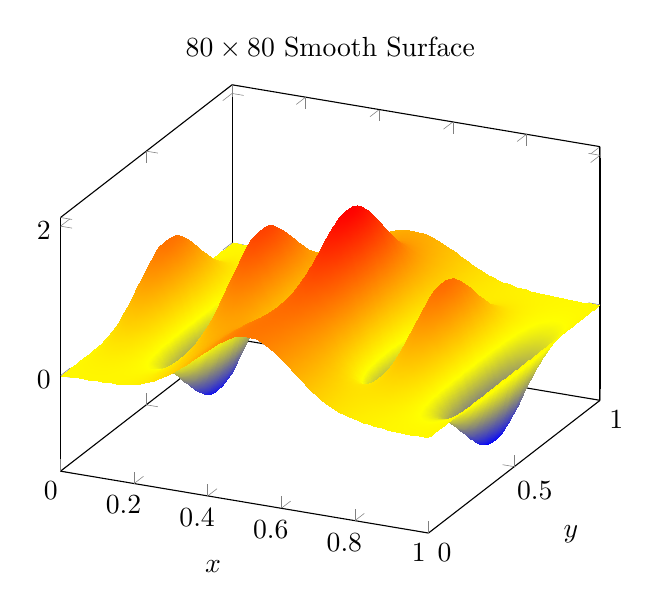
\begin{tikzpicture}
\begin{axis}[
    title=$80 \times 80$ Smooth Surface,
    xlabel=$x$,
    ylabel=$y$,
]
  \addplot3 [surf,samples=80,shader=interp,domain=0:1]
        {sin(deg(8*pi*x))* exp(-20*(y-0.5)^2)
        + exp(-(x-0.5)^2*30
            - (y-0.25)^2 - (x-0.5)*(y-0.25))};
\end{axis}
\end{tikzpicture}
\end{codeexample}

\PGFPlots{} relies completely on \TeX{} to do all typesetting. It uses the
front-end-layer and basic layer of \PGF{} to perform all drawing operations.
For complicated plots, this may take some time, and you may want to read
Chapter~\ref{cha:pgfplots:importexport} for how to write single figures to
external graphics files. Externalization is the best way to reduce typesetting
time.

However, for large scale plots with a lot of points, limitations of \TeX's
capacities are reached easily.


\section{Memory Limitations}

The default settings of most \TeX{} distributions are quite restrictive, so it
may be necessary to adjust them.

Usually, the logfile or the final error message contains a summary about the
used resources, giving a hint which parameter needs to be increased.


\subsection{Lua\LaTeX{}}

One solution which works quite well is to switch the \LaTeX{} executable: if
you have a decent \TeX{} distribution, you will have the |lualatex| executable
as well. This, in turn, uses dynamic memory allocation such that it usually has
enough memory for any \PGFPlots{} axis.

The Lua\LaTeX{} executable |lualatex| is supposed to be almost compatible with
|pdflatex|.

This approach works for any platform.


\subsection{MiK\TeX{}}

If you are running MiK\TeX{} and you do not want to (or cannot switch) to
|lualatex|, you can proceed as follows.

For MiK\TeX{}, memory limits can be increased in two ways. The first is to use
command line switches:
%
\begin{codeexample}[code only]
pdflatex
    --stack-size=n --save-size=n
    --main-memory=n --extra-mem-top=n --extra-mem-bot=n
    --pool-size=n --max-strings=n
\end{codeexample}
%
\noindent Experiment with these settings if MiK\TeX{} runs out of memory.
Usually, one doesn't invoke |pdflatex| manually: there is a development aid
which does all the invocations, so this one needs to be adjusted.

Sometimes it might be better to adjust the MiK\TeX{} configuration file
permanently, for example to avoid reconfiguring the \TeX{} development program.
This can be implemented using the command
%
\begin{codeexample}[code only]
initexmf --edit-config-file=pdflatex
\end{codeexample}
%
\noindent which can be typed either on a command prompt in Windows or using
Start $\gg$ Execute. As a result, an editor will be opened with the correct
config file. A sample config file could be
%
\begin{codeexample}[code only]
main_memory=90000000
save_size=80000
\end{codeexample}
%
or any of the config file entries which are listed below can be entered.
Thanks to ``LeSpocky'' for his documentation in

\url{http://blog.antiblau.de/2009/04/21/speicherlimits-von-miktex-erhoehen}.


\subsection{\TeX{}Live or similar installations}

In addition to the option to switch to |lualatex|, you can proceed as follows
to keep existing |dvips| or |pdflatex| workflows.

For Unix installations, one needs to adjust config files. This can be done as
follows:
%
\begin{enumerate}
    \item Locate |texmf.cnf| on your system. On my Ubuntu installation, it is
        in

        |/usr/share/texmf/web2c/texmf.cnf|.
    \item Either change |texmf.cnf| directly, or copy it to some convenient
        place. If you copy it, here is how to proceed:
        %
        \begin{itemize}
            \item keep only the changed entries in your local copy to
                reduce conflicts. \TeX{} will always read \emph{all} config
                files found in its search path.
            \item Adjust the search path to find your local copy. This can
                be done using the environment variable |TEXMFCNF|. Assuming
                your local copy is in |~/texmf/mytexcnf/texmf.cnf|, you can
                write
                %
\begin{codeexample}[code only]
export TEXMFCNF=~/texmf/mytexcnf:
\end{codeexample}
                %
                to search first in your directory, then in all other system
                directories.
        \end{itemize}
    \item You should change the entries
        %
\begin{codeexample}[code only]
main_memory = n
extra_mem_top = n
extra_mem_bot = n
max_strings = n
param_size = n
save_size = n
stack_size = n
\end{codeexample}
        %
        The logfile usually contains information about the parameter which
        needs to be enlarged.
\end{enumerate}
%
An example of this config file thing is shown below. It changes memory limits.
%
\begin{enumerate}
    \item Create the file |~/texmf/mytexcnf/texmf.cnf| (and possibly the
        paths as well).
        %
\begin{codeexample}[code only]
% newly created file ~/texmf/mytexcnf/texmf.cnf:
% If you want to change some of these sizes only for a certain TeX
% variant, the usual dot notation works, e.g.,
% main_memory.hugetex = 20000000
main_memory = 230000000 % words of inimemory available; also applies to inimf&mp
extra_mem_top = 10000000     % extra high memory for chars, tokens, etc.
extra_mem_bot = 10000000     % extra low memory for boxes, glue, breakpoints, etc.
save_size = 150000    % for saving values outside current group
stack_size = 150000    % simultaneous input sources

% Max number of characters in all strings, including all error messages,
% help texts, font names, control sequences.  These values apply to TeX and MP.
%pool_size = 1250000
% Minimum pool space after TeX/MP's own strings; must be at least
% 25000 less than pool_size, but doesn't need to be nearly that large.
%string_vacancies = 90000
% Maximum number of strings.
%max_strings = 100000
% min pool space left after loading .fmt
%pool_free = 47500
\end{codeexample}
        %
    \item Run |texhash| such that \TeX{} updates its |~/texmf/ls-R| database.
    \item Create the environment variable |TEXMFCNF| and assign the value
        `|~/texmf/mytexcnf:|' (including the trailing `|:|'!). For my linux
        system, this can be done using by adding
        %
\begin{codeexample}[code only]
export TEXMFCNF=~/texmf/mytexcnf:
\end{codeexample}
        %
        to |~/.bashrc|.
\end{enumerate}

Unfortunately, \TeX{} does not allow arbitrary memory limits, there is an upper
bound hard coded in the executables.


\section{Reducing Typesetting Time}

\PGFPlots{} does a lot of computations ranging from abstract coordinate
computations to low level |.pdf| drawing commands (implemented by \PGF{}). For
complex plots, this may take a considerable time -- especially for 3D plots.


\subsection{LUA}

If you use |compat=1.12| (or newer) and compile your documents by means of
|lualatex|, \PGFPlots{} activates its |lua backend|. This switch reduces the
time to generate output files, especially for 3D plots.

\begin{pgfplotskey}{lua backend=\mchoice{true,false} (initially true)}
    If |lua backend| is active and the document is processed by means of
    |lualatex|, \PGFPlots{} activates scalability and performance improvements
    which result in the same output as without it, but with less time and with
    a smarter memory management.

    The feature relies on a partial reimplementation of \PGFPlots{} in the fast
    scripting language \lua. In order to benefit from it, you need to
    %
    \begin{enumerate}
        \item write |compat=1.12| (or newer) into your preamble and
        \item use |lualatex| to translate your |.tex| files (or at least
            those which contain \PGFPlots{} figures).
    \end{enumerate}

    The time to generate surface plots with this feature can be reduced to
    25\%--50\% of the time required by the pure \TeX{} implementation (i.e.\@
    |pdflatex|). Other plot types will also benefit from the feature.

    The |lua backend| works in two ways: first, it substitutes isolated
    routines by faster \lua{} pendants. This is relatively generic. Second, it
    replaces entire processing steps by an equivalent \lua{} implementation.%
    %
    \footnote{
        An example for the first way is: every time \PGFPlots{} makes a lookup
        in its |colormap| it transfers control over to the |lua backend| and
        the result is immediately communicated back to \TeX{}. The main control
        flow resides in the slow \TeX{} implementation. An example for the
        second way is \texttt{\textbackslash addplot expression}: \PGFPlots{}
        will copy the math expression and any related input arguments
        (including \texttt{samples} and \texttt{domain}) over to the
        \texttt{lua backend}. Then, the \texttt{lua backend} will apply all
        loops and collect coordinates which are finally handed over to the
        (\TeX{}) implementation of \pgfname{}. Thus, the control flow resides
        in the fast \lua{} interpreter.
    }
    \PGFPlots{} 1.12 comes with \lua{} implementations for important and
    long-running operations. This implementation will be used whenever
    possible. However, it only covers parts of the feature set: some features
    of \PGFPlots{} are unsupported by the \lua{} backend. In this case, it will
    be switched off automatically and the \TeX{} implementation will be used as
    fallback.

    The |lua backend| will be extended in order to gain more performance
    improvements and in order to cover more features. Please take a look at
    |lua debug| if you want to see if |lua backend| has been (de)activated for
    your figure.

    Note that the |lua backend| uses a different math engine with a higher
    accuracy. As a consequence, the appearance of a plot might have
    insignificant pixel differences compared to the output generated by
    |pdflatex|. It is generally recommended to stick with one way to generate a
    document, i.e.\@ to use either |lualatex| \emph{or} |pdflatex|. Migrating
    from one to another might change the appearance of your document due to
    |lua backend|.

    Eventually, \PGFPlots{} might add computationally expensive features which
    can be implemented as part of |lua backend| and which will be unavailable
    without it.

    Note that |lua backend| requires a \TeX{} distribution which supports at
    least \lua~5.2 (like \TeX{}Live 2014). It will be deactivated
    automatically if your version of |lualatex| is shipped with an older \lua{}
    interpreter.

    Here are some guidelines how to benefit from |lua backend|:
    %
    \begin{itemize}
        \item Math expressions which involve macro definitions are
            unavailable in |lua backend|. Best practice: prefer
            |declare function| over macro constants:
            %
\begin{codeexample}[]
\begin{tikzpicture}
\begin{axis}[
    small,
    title=Do,
    samples=2,
]
    \addplot+ [
        declare function={C=4;}
    ] {C*x};
\end{axis}
\end{tikzpicture}
\end{codeexample}

\begin{codeexample}[]
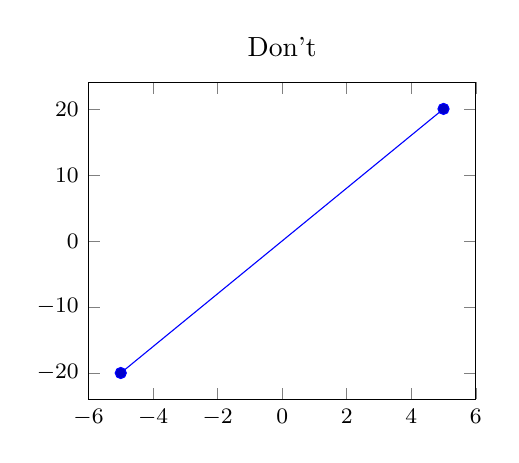
\begin{tikzpicture}
\begin{axis}[
    small,
    title=Don't,
    samples=2,
]
        \def\constantC{4}
    \addplot {\constantC*x};
\end{axis}
\end{tikzpicture}
\end{codeexample}

            Both are semantically equivalent, but since \lua{} cannot interpret
            \TeX{} macros, it refuses to process the ``Don't'' case. The
            ``Don't'' case results in a log message
            %
\begin{verbatim}
Package pgfplots info on input line 16: Deactivating LUA version of
plot expression for plot 0 (type 'pgfplothandlerlineto'):
y expression '\constantC *x' contains a TeX macro.
\end{verbatim}
            %
        \item Any operation which requires ``native'' \TeX{} code is
            unavailable in |lua backend|. This includes
            |x filter/.code={...}| since |/.code| cannot be mapped to \lua.
            Best practice: prefer |x filter/.expression| over |x filter/.code|:
            %
\begin{codeexample}[]
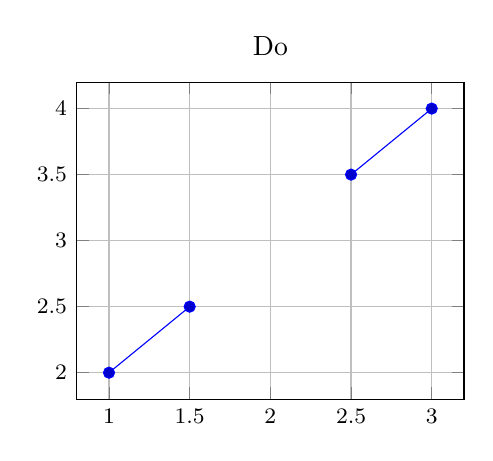
\begin{tikzpicture}
    \begin{axis}[small,grid=major,title=Do]
    \addplot+ [
        unbounded coords=jump,
        y filter/.expression={y==3 ? nan : y},
    ] table {
        x   y
        1   2
        1.5 2.5
        2   3
        2.5 3.5
        3   4
    };
    \end{axis}
\end{tikzpicture}
\end{codeexample}
            %
        \item Plot expression can be processed entirely in \lua, all other
            input coordinate types use \TeX{} to read the value and hand-over
            to \lua.
        \item There are a couple of operations for which the |lua backend| is
            planned for future releases.
    \end{itemize}
\end{pgfplotskey}

\begin{pgfplotskeylist}{%
    lua debug,
    lua debug=\mchoice{false,off,off and silent,verbose,compileerror}%
}
    Typically, the |lua backend| works silently: \PGFPlots{} decides if it is
    active and if it supports the current operation and proceeds accordingly.
    If both conditions are satisfied, it will transfer control to the
    |lua backend|. If one of them is not met, it will automatically fall back
    to the old \TeX{} implementation. As a consequence, it cannot be sensed
    right away, only the time to compile pictures will vary.

    This key controls how \PGFPlots{} handles the case where the |lua backend|
    is active, but cannot be used because some encountered feature is
    unsupported.

    The choices \declaretext{false} and \declaretext{off} deactivate \lua{}
    debugging. In this case, \PGFPlots{} will \emph{only} write log messages if
    it used the \TeX{} implementation instead of the |lua backend|. In
    addition, it will only write the messages into the |.log| file (but not
    into the console output).

    The choice \declaretext{off and silent} writes neither information messages
    nor debug messages: it is the same as |off| but without the log message if
    the \TeX{} implementation has been used. It is the least verbose choice.

    The choice \declaretext{verbose} will also write success messages into the
    |.log| file (not into the console).

    The choice \declaretext{compileerror} will abort compilation if the
    |lua backend| is active but does not support the current figure or plot.

    Note that \PGFPlots{} might come with limited expensive operations which
    are only available in the |lua backend|. These items will result in compile
    errors if the |lua backend| cannot be used for some reason.
\end{pgfplotskeylist}


\subsection{Compiling Images Just Once}

One possibility to reduce typesetting time is to tell \PGF{} to generate
single, temporary |.pdf| (or |.eps|) documents for a subset (or all) graphics
in one run and reuse these temporary images in successive runs. For
\PGFPlots{}, this is the most effective way to reduce typesetting time for
larger documents. It can be accomplished using the |external| library described
in Section~\ref{sec:pgfplots:export}.

}
